\documentclass[a4paper]{article}
\usepackage[italian]{babel}

% immagini
\usepackage{graphicx}
\usepackage{svg}
\usepackage{amsthm}
\usepackage{geometry}
\usepackage{subcaption}
% matematica
\usepackage{amsmath}
\usepackage{amsfonts}
\usepackage{unicode-math}

% codice
\usepackage{listings}
\lstset{
    basicstyle=\small\ttfamily,
    numbers=left,
    numberstyle=\small\ttfamily
}

% \usepackage{blindtext}
\usepackage{titlesec}
% \usepackage{geometry}
% \usepackage{relsize}
\usepackage{tikz}
% \geometry{
% a4paper,
% total={190mm,257mm},
% left=25mm,
% right=25mm,
% top=50mm,
% }
\geometry{a4paper, margin=1in} % Set margins to fit the entire content better
\usepackage{hyperref}

% \sloppy % ?

% comandi per riferirsi agli algoritmi
\newcommand{\QuickSelect}{\textsc{QuickSelect}}
\newcommand{\HeapSelect}{\textsc{HeapSelect}}
\newcommand{\MoMSelect}{\textsc{MoMSelect}}

% comandi per la notazione asintotica
\newcommand{\Tquad}{\ifmmode \Theta(n^2) \else $\Theta(n^2)$\fi} % Θ(n^2)
\newcommand{\Tlin}{\ifmmode \Theta(n) \else $\Theta(n)$\fi} % Θ(n)
\newcommand{\Olin}{\ifmmode O(n) \else $O(n)$\fi} % O(n)

\begin{document}

\begin{titlepage} % pagina riservata al titolo
    \begin{center}
        \vspace*{1cm}
        {\Huge\bfseries Analisi di algoritmi di selezione\par}
        \vspace{.5cm}
        {\LARGE Progetto di laboratorio di Algoritmi e Strutture Dati\par}
        \vspace{1cm}
        \begin{figure}[h]
            \centering
            
\includegraphics[width=.5\textwidth]{photo/uniud_logo.png}
        \end{figure}
        \vspace{1.5cm}
        {\LARGE Università degli studi di Udine\par}
        {\LARGE Dipartimento di scienze Informatiche, Matematiche e Fisiche\par}
        \vfill
        {\Large Anno Accademico 2023/2024\par}
        {\Large Matricole: 162367, 162013, 162473\par}
        {\Large\itshape Gerardi Ludovico, Sclauzero Lorenzo, Pantanali Riccardo\par}
    \end{center}
\end{titlepage}



\section{Introduzione}
Il progetto ha come scopo l'implementazione di tre algoritmi di selezione e l'analisi della loro complessità.
Dato un vettore di interi $v$ di dimensione $n$ e un intero $k$ con $1 < k \le n$, gli algoritmi di selezione calcolano il $k$-esimo elemento più piccolo di $v$.

I tre algoritmi discussi sono \QuickSelect{}, \HeapSelect{} e \MoMSelect{} (che sta per median-of-medians select); vengono presentati nella sezione \ref{sec:presentazione-algoritmi} insieme all'algoritmo utilizzato per la generazione dell'input.
Nella sezione \ref{sec:misurazione} si discute brevemente la misurazione dei tempi di esecuzione, necessaria per l'analisi della complessità.
Nella sezione \ref{sec:grafici} vengono presentati e discussi i risultati delle misurazioni sotto forma di grafici.
Infine nella sezione \ref{sec:confronto-mom} viene proposto un confronto tra alcune varianti di \MoMSelect{}.



\section{Presentazione degli algoritmi}
\label{sec:presentazione-algoritmi}

\subsection{Algoritmi di selezione}
\paragraph{\QuickSelect}
Questo algoritmo partiziona ricorsivamente $v$ rispetto a un elemento scelto come pivot e confronta la posizione finale del pivot con $k$: sono sono uguali allora l'algoritmo termina, ritornando $v[k]$; altrimenti effettua una chiamata ricorsiva sulla partizione sinistra o destra di $v$, a seconda che $k$ sia rispettivamente minore o maggiore della posizione finale del pivot.
Quest'ultimo viene scelto sempre come l'ultimo elemento del sottovettore considerato.
Tale approccio porta la complessità nel caso peggiore a essere \Tquad{} (quando il vettore è già ordinato, in un senso o nell'altro), mentre nel caso medio è \Tlin.
D'altra parte l'overhead dovuto alla scelta del pivot è molto basso, il che, come si vedrà, porta ad un vantaggio rispetto a \MoMSelect{} nel caso di vettore generati pseudocasualmente.

\paragraph{\HeapSelect}
\HeapSelect{} utilizza due heap $H_1$ e $H_2$.
$H_1$ è una min-heap che viene costruita a partire da $v$ in tempo lineare e non viene successivamente modificata.
$H_2$ è una min-heap che inizialmente contiene solo il nodo radice di $H_1$.
Ad ogni iterazione viene estratta la radice $r$ da $H_2$ e vengono aggiunti i figli di $r$ in $H_1$ all'interno di $H_2$.
Dopo $k-1$ iterazioni $r$ è l'elemento cercato, cioè il $k$-esimo più piccolo all'interno di $v$.
Siccome cercare il $k$-esimo elemento più piccolo equivale a cercare l'elemento $(n-k+1)$-esimo più grande, se $k>n/2$ è si utilizza una max-heap per $H_2$, il che consente di ridurre il numero di iterazioni necessarie.
Questo algoritmo ha una complessità temporale pari a $O(n+k\log k)$ sia nel caso pessimo che in quello medio.

\paragraph{\MoMSelect}
Il funzionamento ad alto livello di \MoMSelect è come quello di \QuickSelect: effettuare una chiamata ricorsiva sulla porzione di vettore che contiene l'elemento cercato.
La differenza tra i due algoritmo sta nella scelta del pivot.
Infatti \MoMSelect{} utilizza una procedura ausiliaria che calcola la posizione della mediana delle mediana all'interno del sottovettore considerato.
Nello specifico tale procedura divide il vettore in blocchi da $5$ elementi (eccetto al più l'ultimo blocco), ordina ciasun blocco e ne calcola la mediana, e quindi effettua una chiamata ricorsiva sulle mediane appena calcolate finché non rimane un solo elemento: la mediana delle mediane.
Sono proposte due varianti:
\begin{enumerate}
    \item non in-place: alloca un nuovo vettore ad ogni chiamata ricorsiva per memorizzare le mediane dei blocchi;
    \item quasi in-place: riutilizza lo spazio allocato per il vettore originariamente fornito in input;
    \item in-place: non utilizzando le chiamate ricorsive;
\end{enumerate}

In tutti i casi, la complessità temporale e spaziale dell'algoritmo nel caso pessimo è \Olin.
Nei grafici della sezione \ref{sec:grafici} verrà utilizzata la versione quasi in-place.

\subsection{Algoritmo per la generazione dei vettori}
La lunghezza $n$ del vettori generati varia da $1000$ ($n_{\min}$) a $100000$ ($n_{\max}$), mentre i valori degli interi variano $0$ a $100000$.
In certe misurazioni la lunghezza dei vettori cresce secondo la serie geometrica
\[
    L(i) = n_{\min} \cdot \left(\frac{n_{\max}}{n_{\min}}\right)^{i/99}
\]
dove $i$ è il numero dell'iterazione corrente, che varia da $0$ a $99$, per un totale di $100$ iterazioni.
Si noti in particolare che $L(0) = n_{\min}$ e $L(99) = n_{\max}$.


\section{Misurazione dei tempi di esecuzione}
\label{sec:misurazione}
La misurazione dei tempi necessari per calcolare il k-esimo numero in un array viene effettuata considerando la lunghezza \( n \) dell'array di input e l'errore massimo consentito. Per ogni lunghezza dell'array, gli algoritmi implementati ripetono il calcolo del k-esimo numero un numero di volte tale da garantire un errore massimo relativo pari a \( f_{\max} = 0.001 \), assicurando così un tempo totale maggiore o uguale a \( T_{\min} \), calcolato come \[ T_{\min} = R \left( \frac{1}{f} + 1 \right) \] dove \( R \) rappresenta la risoluzione del clock.

Ciascuna iterazione del calcolo del k-esimo numero viene eseguita su un array generato pseudo-casualmente di lunghezza \( n \), differente ad ogni iterazione.
L'analisi dell'efficienza dei tre algoritmi viene effettuata attraverso la misurazione dei tempi medi\\

\newpage

\section{Rappresentazione grafica dei risultati}
\label{sec:grafici}
\begin{figure}[h]
            \centering
            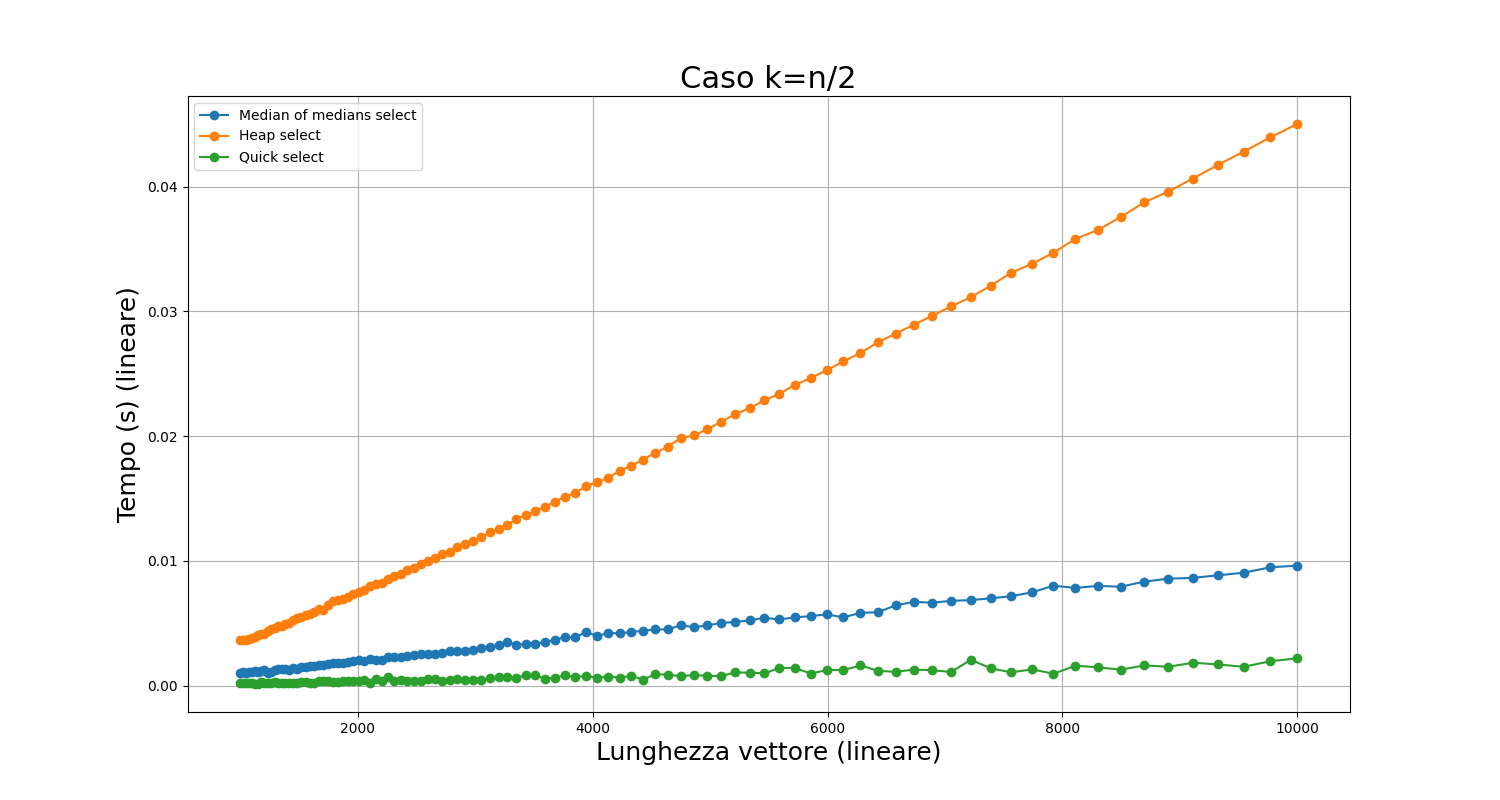
\includegraphics[width=.83\textwidth]{graphs/k_const_n.png}
            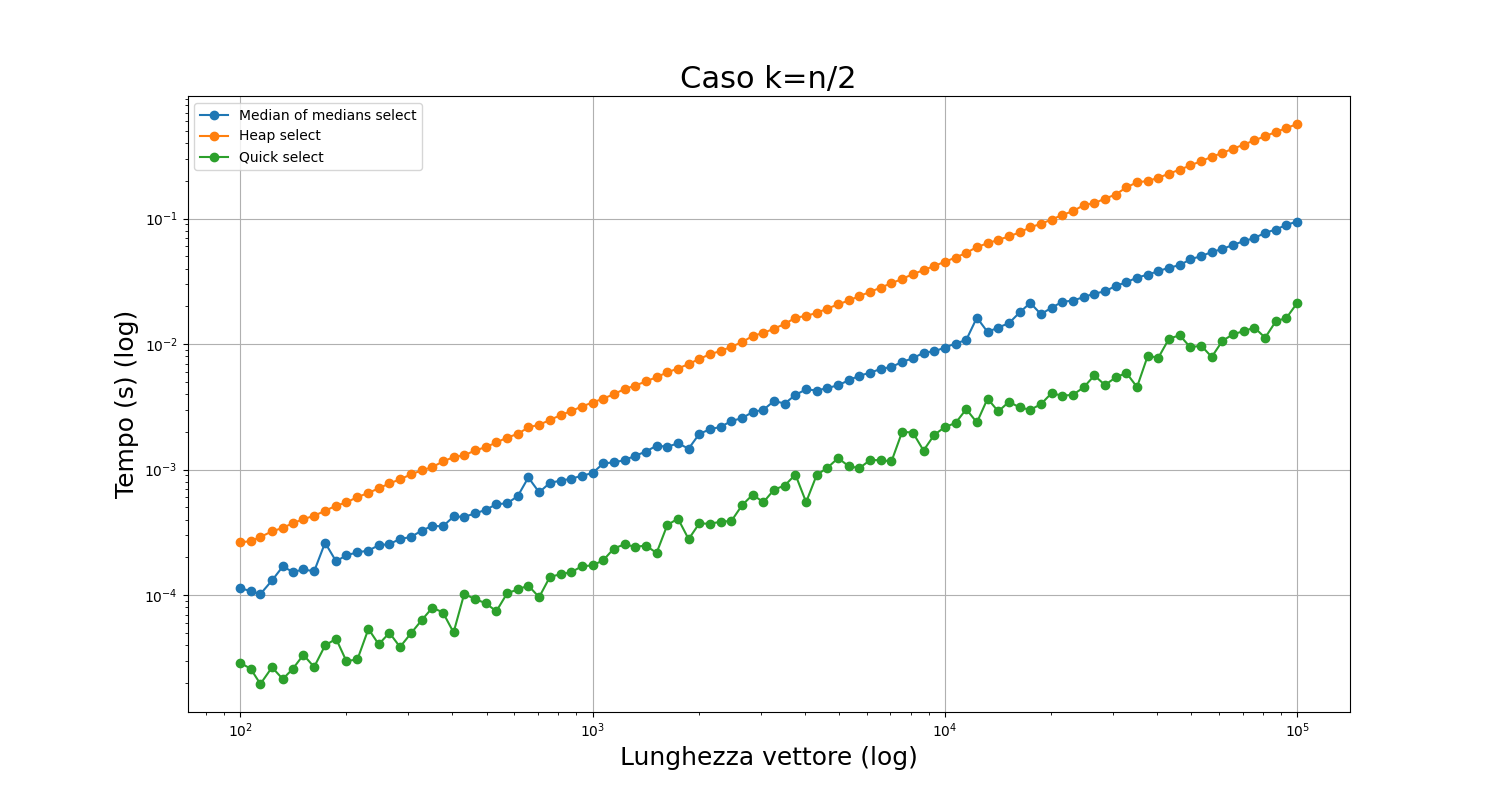
\includegraphics[width=.83\textwidth]{graphs/k_const_2xlog.png}
\end{figure}
Come evidenziato dai grafici, nel caso in cui $k=n/2$ l'algoritmo \HeapSelect{} è più inefficiente rispetto a \QuickSelect{} e \MoMSelect{}.
Per spiegare questo comportamento occorre tenere conto della complessità di \HeapSelect{}; infatti sostituendo $k$ con $n/2$ nella formula della complessità di ottiene:
\[\begin{split}
	O(n + k\log k) 	& = O\left(n + \frac{n}{2}\log \frac{n}{2}\right) \\
			& = O\left(n + \frac{n}{2}(\log n - \log 2)\right) \\
			& = O\left(n + \frac{n}{2}\log n - \frac{n}{2}\log 2\right) \\
			& = O(n \log n)
\end{split}\]
cioè la crescita di \HeapSelect{} risulta superlineare.
È facile vedere che lo stesso risultato si ottiene ogni volta che $k$ è una frazione di $n$.

Invece \MoMSelect{} e \QuickSelect{} hanno entrambi complessità $O(n)$.
Tuttavia \QuickSelect{} risulta più veloce rispetto a \MoMSelect{} e ciò è dovuto all'overhead richiesto da quest'ultimo algoritmo per calcolare la mediana delle mediane.

\newpage
\subsection{Caso k estremo}
\begin{figure}[h]
            \centering
            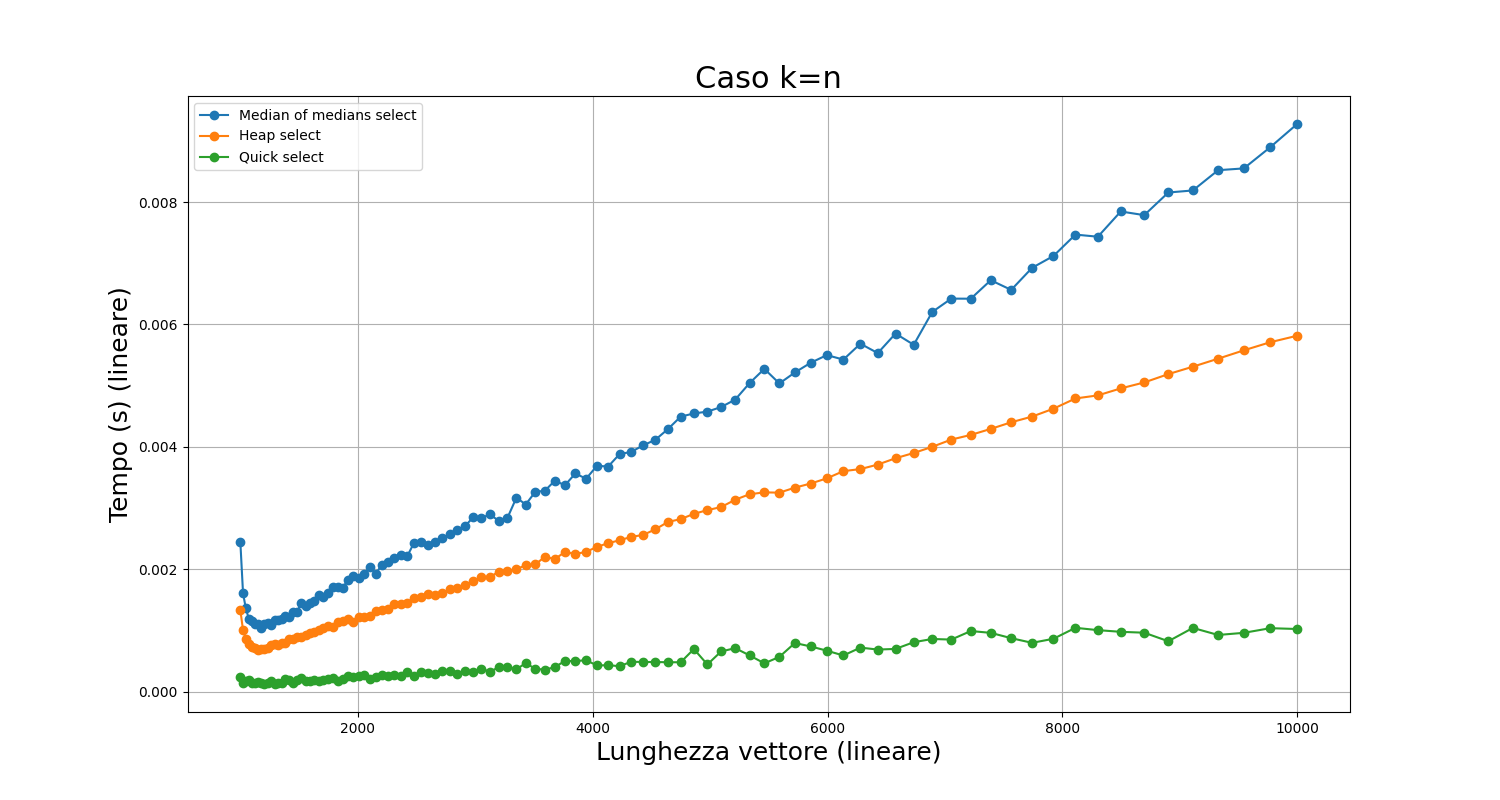
\includegraphics[width=.83\textwidth]{graphs/k_last_n.png}
            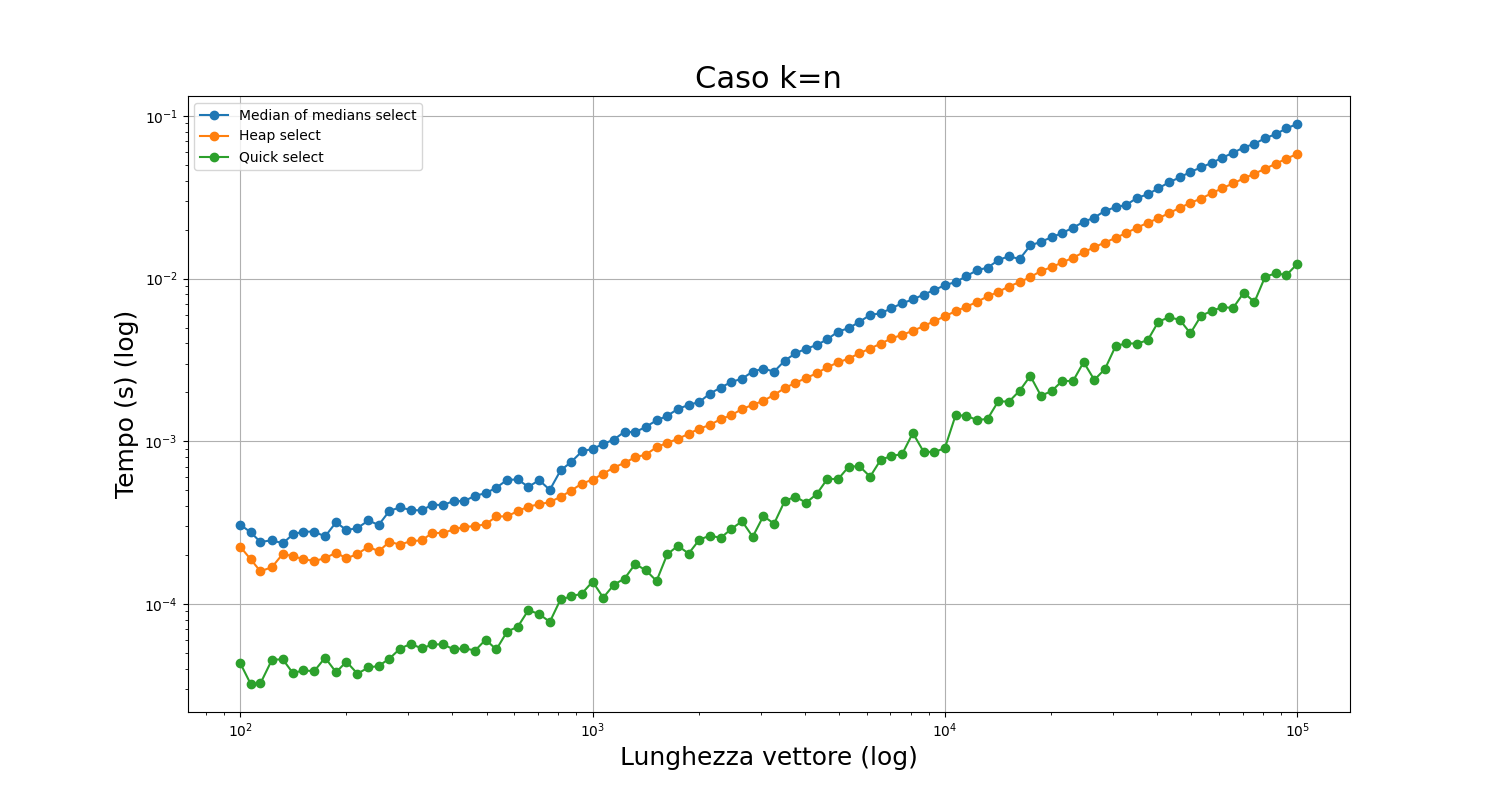
\includegraphics[width=.83\textwidth]{graphs/k_last_2xlog.png}
\end{figure}
Nel caso in cui $k$ sia un estemo del vettore, cioè $k=1$ o $k=n$, si nota un netto miglioramento da parte di \HeapSelect{}, tanto da diventare migliore di \MoMSelect{}.
Infatti essendo $k$ costante l'apporto dato dal fattore $k\log k$ diventa trascurabile e quindi il costo di \HeapSelect{} diventa $O(n)$; tale costo è per la maggior parte dovuto alla costruzione dell'heap.
Possiamo quindi affermare che questa operazione risulta più veloce, seppure di poco, rispetto al calcolo della mediana della mediane.
Notiamo che siccome per $k > n/2$ si utilizza una max heap, il costo nel caso in cui $k=n$ è pari a quello in cui $k=1$.

Per quanto riguarda \QuickSelect{} e \MoMSelect{}, il loro andamento risulta praticamente invariato rispetto al caso precedente.


\newpage
\subsection{Caso k random}
\begin{figure}[h]
            \centering
            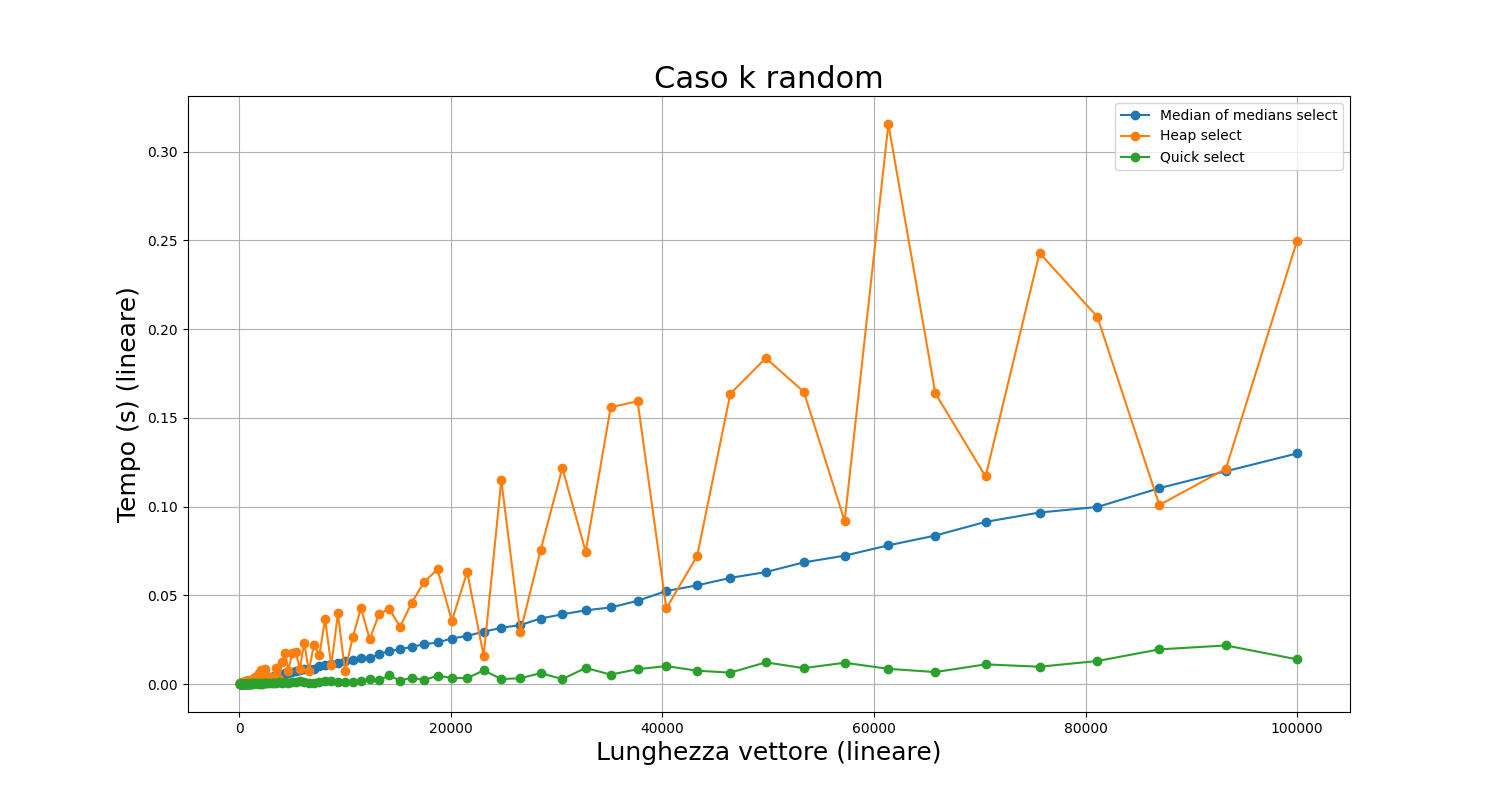
\includegraphics[width=.83\textwidth]{graphs/k_random_n.png}
            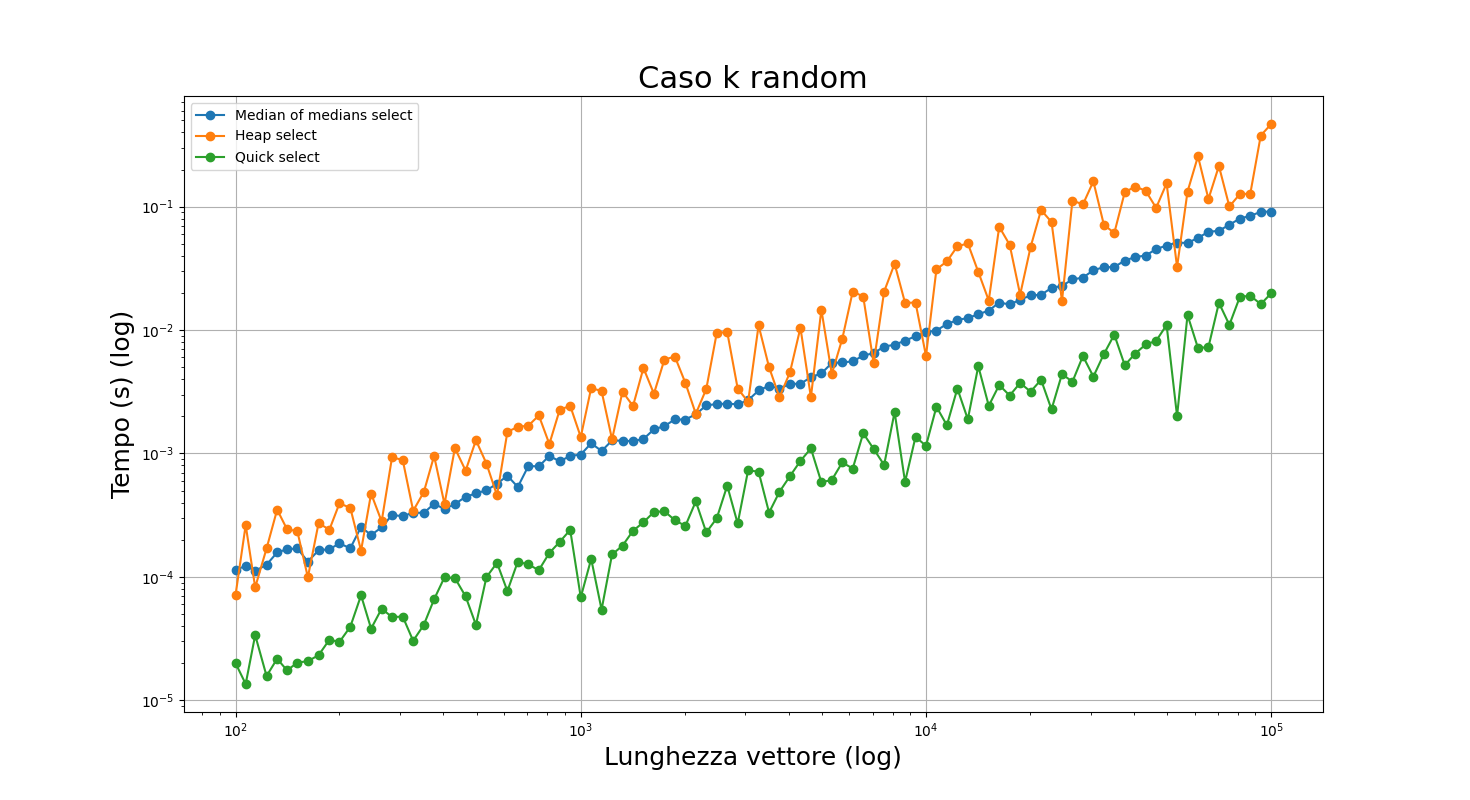
\includegraphics[width=.83\textwidth]{graphs/k_random_2xlog.png}
\end{figure}

Nel caso in cui $k$ sia casuale emerge chiaramente l'indipendenza dell'algoritmo \MoMSelect{} da $k$: il suo andamento risulta infatti molto stabile al variare di $k$, e ciò è da attribuirsi al calcolo della mediana delle mediane, che assicura un andamento lineare.

Invece \HeapSelect{} mostra un andamento più instabile.
Ciò è dovuto al fatto che $k$ determina la sue complessità complessità, che varia da $O(n)$ a $O(n\log n)$, come si è già visto.

Anche \QuickSelect{} si mostra più instabile di \MoMSelect{}.
Ricordiamo infatti che nel caso peggiore la complessità di \QuickSelect{} è $\Theta(n^2)$.



\newpage
\subsection{Caso n fissato e k variato}
\begin{figure}[h]
    \centering
    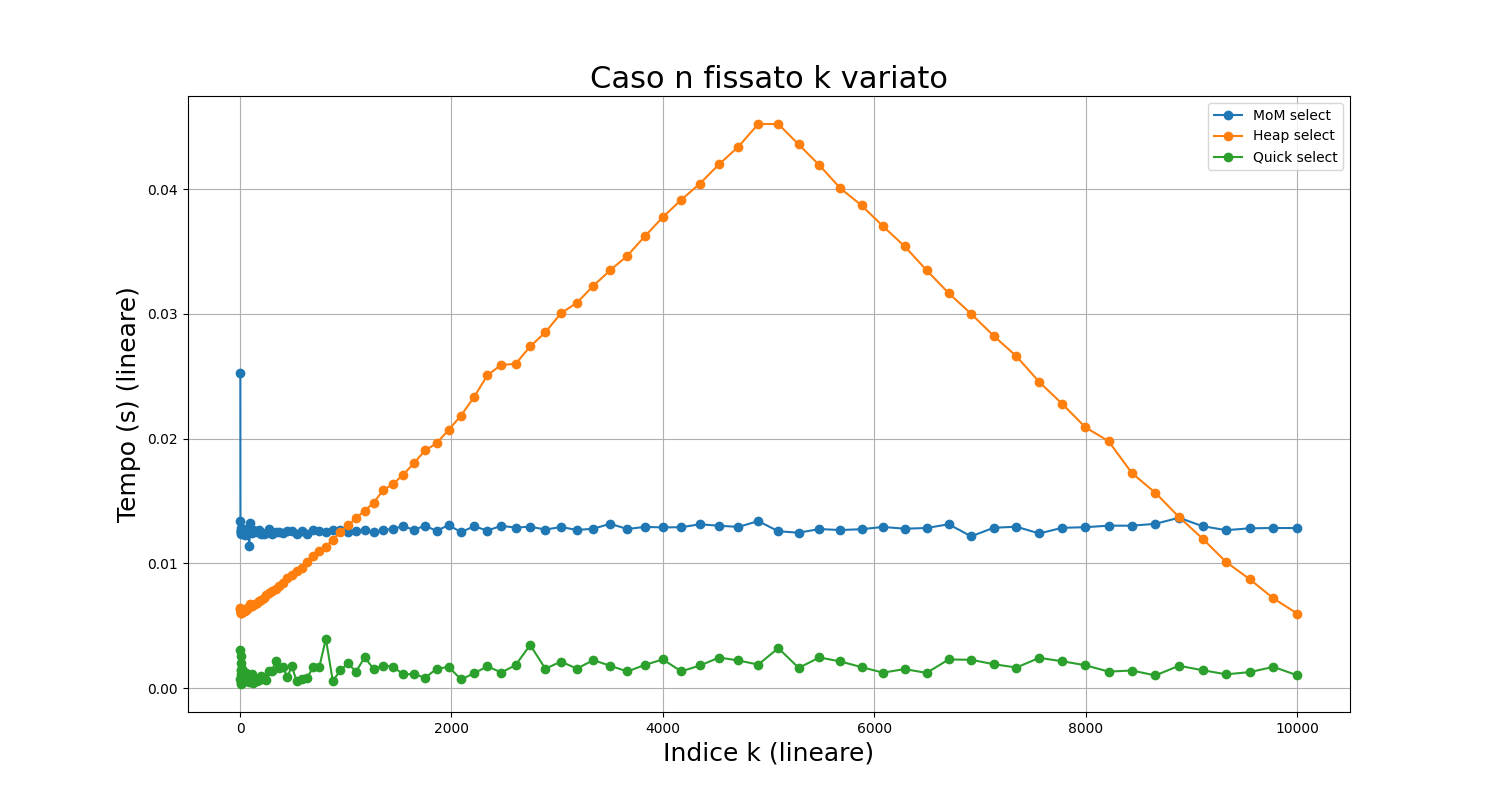
\includegraphics[width=.83\textwidth]{graphs/n_fixed_n.png}
    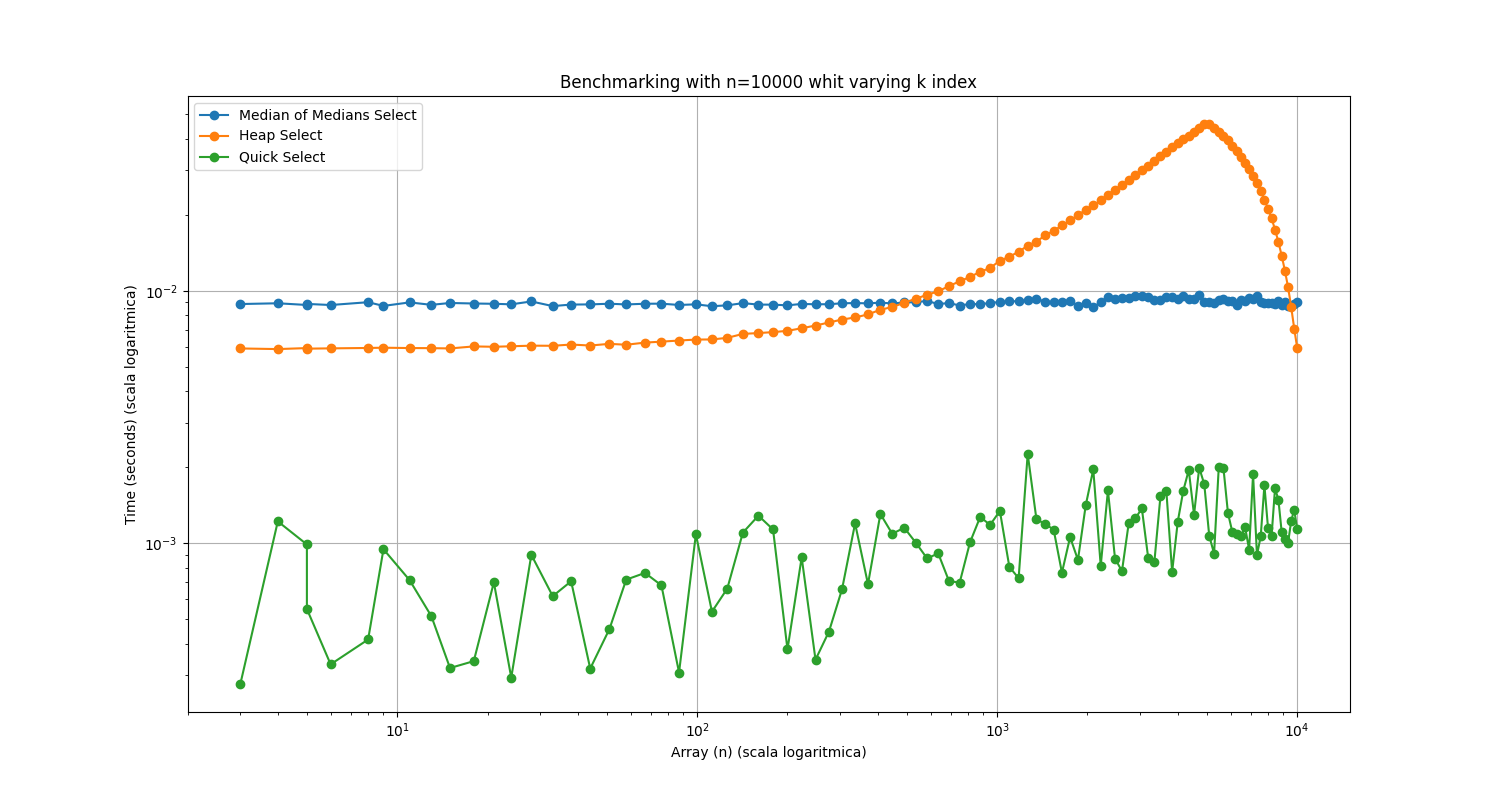
\includegraphics[width=.83\textwidth]{graphs/n_fixed_2xlog.png}
\end{figure}

In questo caso la lunghezza di $n$ è fissata a $10000$ e $k$ varia in $[1,\dots,10000]$.
Risulta evidente la dipendenza di \HeapSelect{} dallo stesso.
Dal suo andamento piramidale risulta chiaro come il tempo di esecuzione cresca monotonicamente fino a $k=n/2$ e poi decresca monotonicamente.
Ciò è ovviemente dovuto al fatto che l'implementazione utilizza una max heap per $k>n/$; se non fosse così è facile immaginare che il tempo continuerebbe a crescere dopo $n/2$.

Riguardo a \QuickSelect{} e \MoMSelect{} non traspare nulla di differente da quello che abbiamo già evidenziato nelle sezioni precedenti.

\newpage
\subsection{Caso peggiore per \QuickSelect}
\begin{figure}[h]
    \centering
    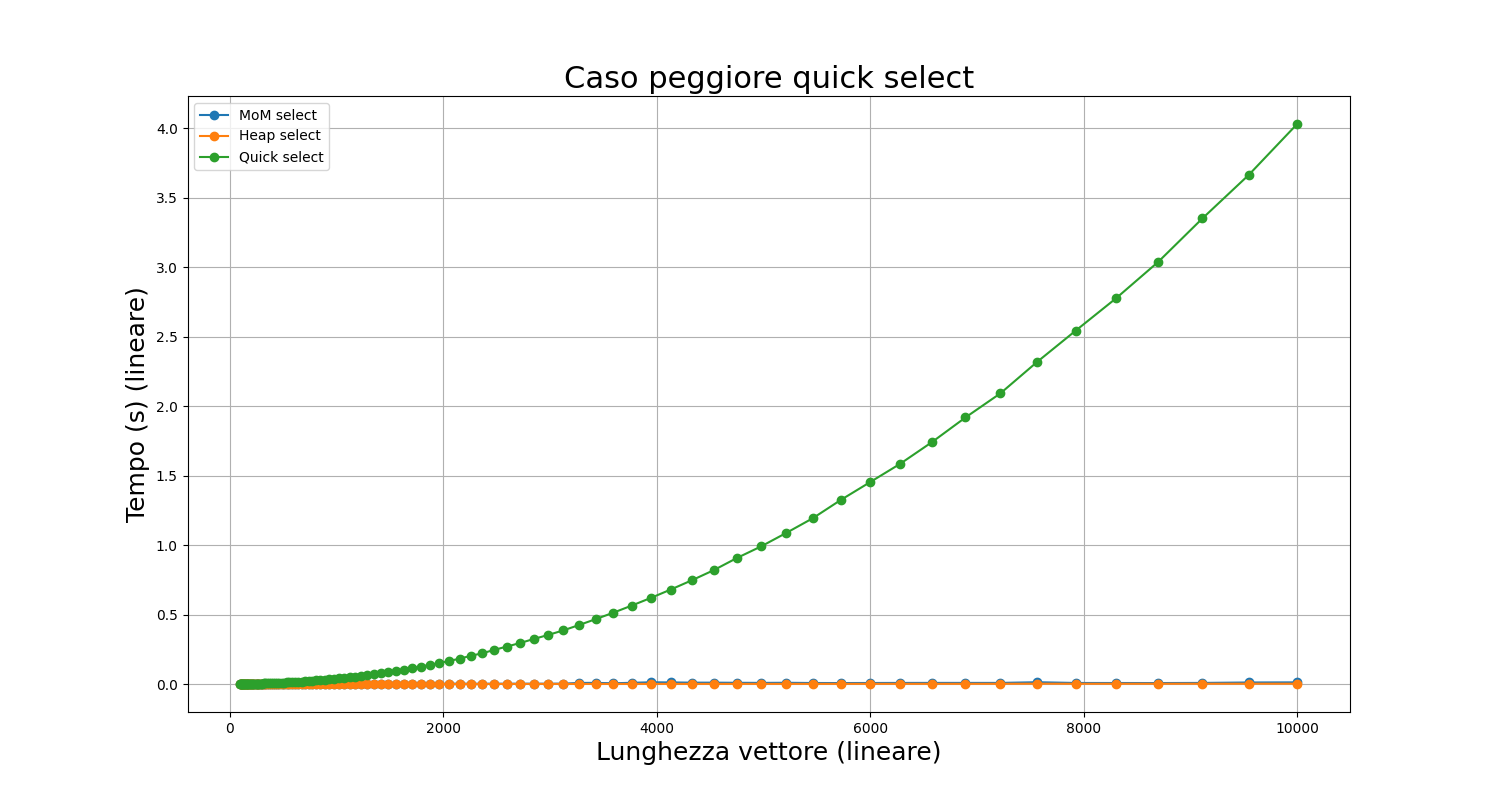
\includegraphics[width=.83\textwidth]{graphs/QS_wrost_case.png}
    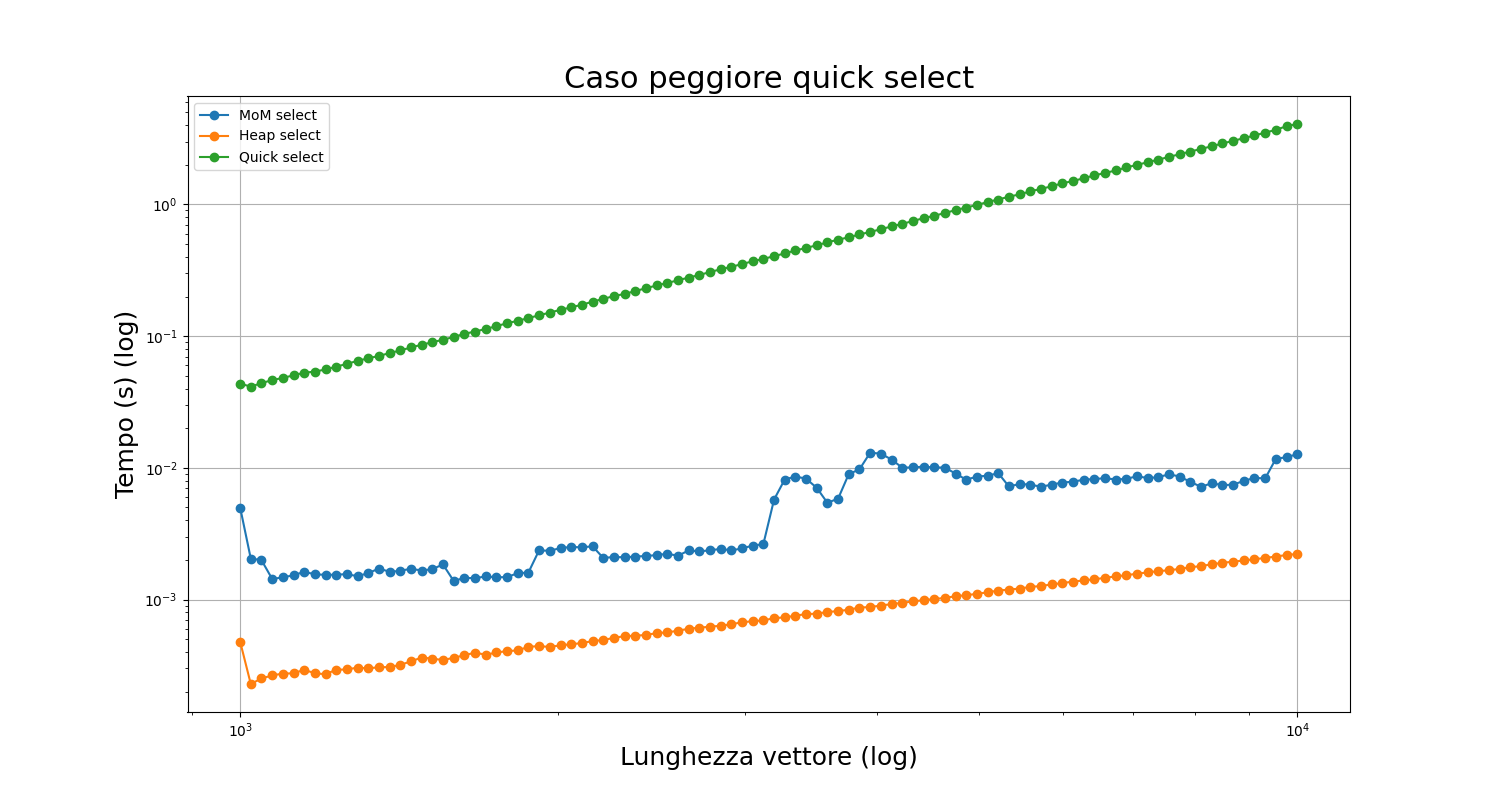
\includegraphics[width=.83\textwidth]{graphs/QS_2xlog.png}
\end{figure}
Dai casi precedenti si è visto come \QuickSelect{}, nonostante abbia nel caso peggiore una complessità $\Tquad$, difatto con un vettore generato pseudocasualemente risulti essere migliore di \HeapSelect{} e \MoMSelect{}, e quindi può essere un buon candidato come algoritmo di selezione se si è ragionevolmente sicuri che il caso peggiore non possa verificarsi.
Ma vediamo ora due casi in cui ciò può accadere: il primo in cui il vettore è ordinato in modo crescente e $k=1$ ovvero quello rappresentato dai grafici soprastanti mentre il secondo in cui il vettore è ordinato in modo decrescente e $k=n$ che però nel nostro caso non risulta essere il peggiore. Questo è dovuto dal fatto che nel nostro codice il pivot risulta essere sempre l'ultimo elemento della porzione. Di conseguenza il pivot scelto è sempre l'elemento più piccolo della porzione corrente dell'array, ma poiché stiamo cercando l'elemento più grande, lo troviamo subito senza dover iterare attraverso tutte le partizioni\\


\newpage

\section{Confronto tra MoM}
\label{sec:confronto-mom}
\begin{figure}[h]
    \centering
    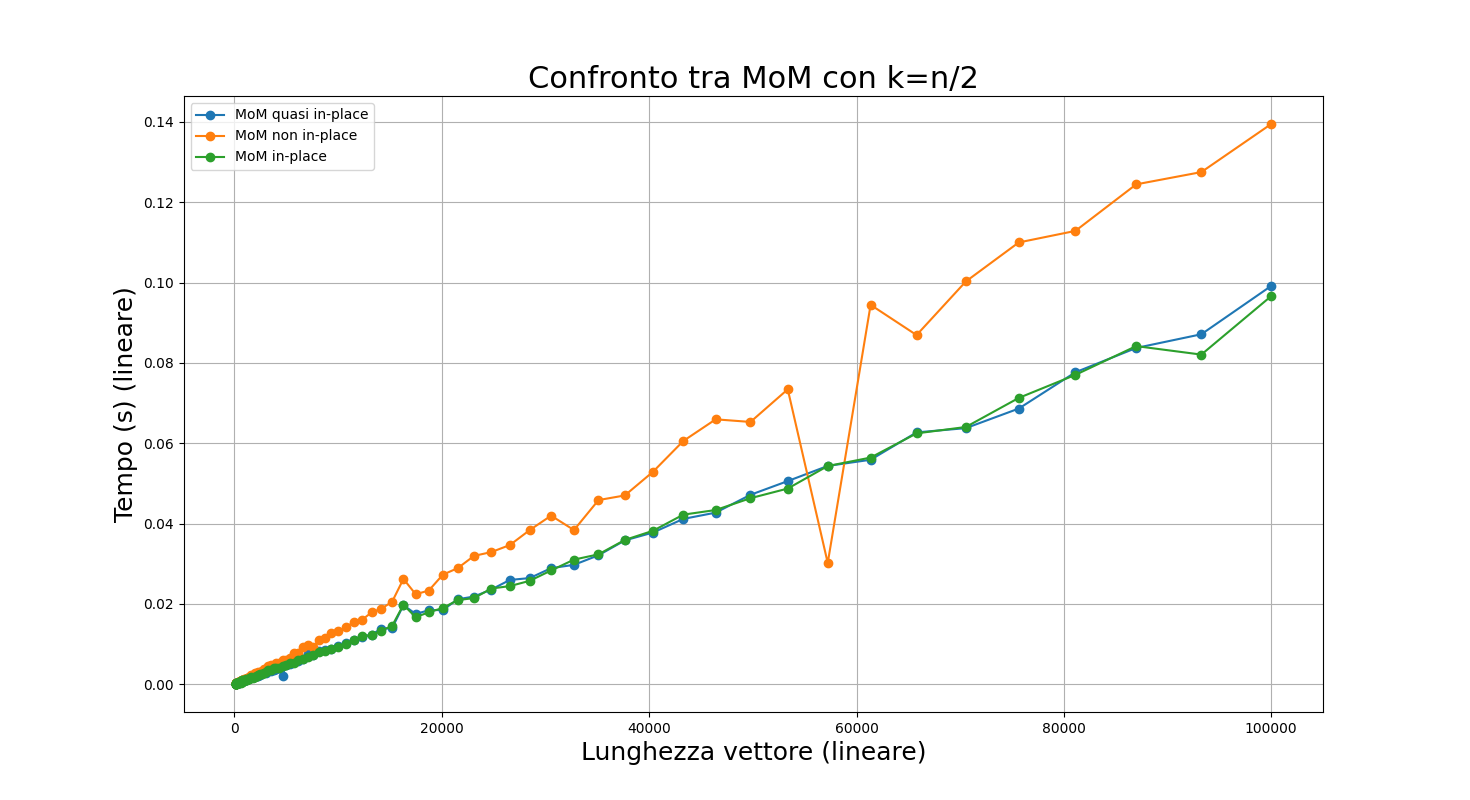
\includegraphics[width=.83\textwidth]{graphs/MoMs_n.png}
    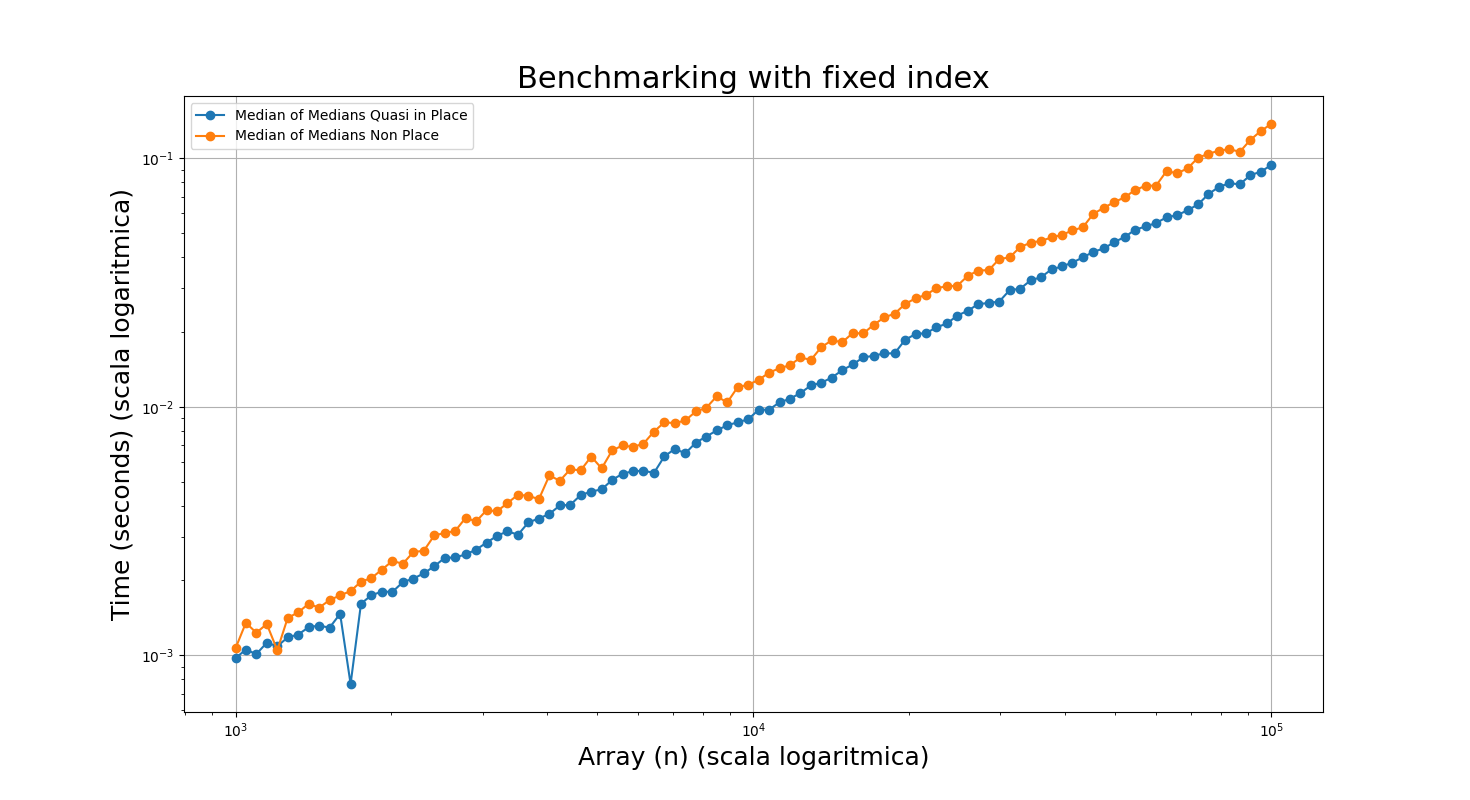
\includegraphics[width=.83\textwidth]{graphs/MoMs_2xlog.png}
\end{figure}
Come si può notare i tre algoritmi hanno degli andamenti molto simili, avendo una complessità $O(n)$. La versione non in place a causa delle chiamate ricorsive e dell'utilizzo di due array supplementari si rivela essere meno prestante al crescere della lunghezza dell'array.\\
\end{document}
